%%%%%%%%%%%%%%%%%%%%%%%%%%%%%%%%%%%%%%%%%%%%%%%%%%%%%%%%%%%%%%%%%%%%%%%%%%%%%%%%
%
% Template license:
% CC BY-NC-SA 3.0 (http://creativecommons.org/licenses/by-nc-sa/3.0/)
%
%%%%%%%%%%%%%%%%%%%%%%%%%%%%%%%%%%%%%%%%%%%%%%%%%%%%%%%%%%%%%%%%%%%%%%%%%%%%%%%%

%----------------------------------------------------------------------------------------
%	PACKAGES AND OTHER DOCUMENT CONFIGURATIONS
%----------------------------------------------------------------------------------------

\documentclass[
11pt, % The default document font size, options: 10pt, 11pt, 12pt
%oneside, % Two side (alternating margins) for binding by default, uncomment to switch to one side
%chapterinoneline,% Have the chapter title next to the number in one single line
spanish,
singlespacing, % Single line spacing, alternatives: onehalfspacing or doublespacing
%draft, % Uncomment to enable draft mode (no pictures, no links, overfull hboxes indicated)
%nolistspacing, % If the document is onehalfspacing or doublespacing, uncomment this to set spacing in lists to single
%liststotoc, % Uncomment to add the list of figures/tables/etc to the table of contents
%toctotoc, % Uncomment to add the main table of contents to the table of contents
parskip, % Uncomment to add space between paragraphs
%codirector, % Uncomment to add a codirector to the title page
headsepline, % Uncomment to get a line under the header
sidewaystable
lscape
]{MastersDoctoralThesis} % The class file specifying the document structure

\usepackage{lscape}
\usepackage{multirow}
\usepackage{float}
\renewcommand{\labelenumii}{\arabic{enumi}.\arabic{enumii}}
\renewcommand{\labelenumiii}{\arabic{enumi}.\arabic{enumii}.\arabic{enumiii}}
\renewcommand{\labelenumiv}{\arabic{enumi}.\arabic{enumii}.\arabic{enumiii}.\arabic{enumiv}}

%----------------------------------------------------------------------------------------
%	INFORMACIÓN DE LA MEMORIA
%----------------------------------------------------------------------------------------

\thesistitle{Reconocimiento de intrusos en video de vigilancia aérea} % El títulos de la memoria, se usa en la carátula y se puede usar el cualquier lugar del documento con el comando \ttitle

% Nombre del posgrado, se usa en la carátula y se puede usar el cualquier lugar del documento con el comando \degreename
%\posgrado{Carrera de Especialización en Inteligencia Artificial} 
%\posgrado{Carrera de Especialización en Internet de las Cosas} 
\posgrado{Carrera de Especialización en Inteligencia Artificial}
%\posgrado{Maestría en Sistemas Embebidos} 
%\posgrado{Maestría en Internet de las cosas}

\author{Ing. Juan Pablo Nieto Uribe} % Tu nombre, se usa en la carátula y se puede usar el cualquier lugar del documento con el comando \authorname

\director{Esp. Ing. Hernán Contigiani (FIUBA)} % El nombre del director, se usa en la carátula y se puede usar el cualquier lugar del documento con el comando \dirname
\codirector{Nombre del codirector (pertenencia)} % El nombre del codirector si lo hubiera, se usa en la carátula y se puede usar el cualquier lugar del documento con el comando \codirname.  Para activar este campo se debe descomentar la opción "codirector" en el comando \documentclass, línea 23.

\juradoUNO{Dr. Ing. Leonardo Alfredo Forero Mendoza (PUC-RIO)} % Nombre y pertenencia del un jurado se usa en la carátula y se puede usar el cualquier lugar del documento con el comando \jur1name
\juradoDOS{Dr. Ing. Javier Andrés Redolfi (UTN - FRSF)} % Nombre y pertenencia del un jurado se usa en la carátula y se puede usar el cualquier lugar del documento con el comando \jur2name
\juradoTRES{Ing. Juan Ignacio Cavalieri (DeepAgro)} % Nombre y pertenencia del un jurado se usa en la carátula y se puede usar el cualquier lugar del documento con el comando \jur3name

%\ciudad{Ciudad Autónoma de Buenos Aires}
%\ciudad{ciudad de Mendoza}
\ciudad{ciudad de Bogotá, Colombia}

\fechaINICIO{octubre de 2021}
\fechaFINAL{junio de 2023}


\keywords{Inteligencia artificial, FIUBA,dron, vigilancia} % Keywords for your thesis, print it elsewhere with \keywordnames


\begin{document}


\frontmatter % Use roman page numbering style (i, ii, iii, iv...) for the pre-content pages

\pagestyle{plain} % Default to the plain heading style until the thesis style is called for the body content


%----------------------------------------------------------------------------------------
%	RESUMEN - ABSTRACT 
%----------------------------------------------------------------------------------------

\begin{abstract}
\addchaptertocentry{\abstractname} % Add the abstract to the table of contents
%
%The Thesis Abstract is written here (and usually kept to just this page). The page is kept centered vertically so can expand into the blank space above the title too\ldots
\centering

La presente memoria detalla el proceso de creación de un módulo de inteligencia artificial, diseñado para implementar un sistema de detección de personas y animales de gran porte de forma que sea posible automatizar el proceso de vigilancia y así reducir el personal encargado a esta labor, y permitiendo abaratar costos y aumentar la precisión en el proceso. En particular, lo que se pretende con el desarrollo de este trabajo es detectar intrusos en \textit{streaming} de vídeo tomado desde un dron, como parte de un sistema más grande de vigilancia, que será implementado por la empresa Manta Beach. Esta empresa, que hace parte del programa de vinculación de la universidad, propuso el trabajo como parte de su plan de investigación y desarrollo.

Para la creación de este módulo, se hace un uso extensivo de los conocimientos de la rama de visión por computadora a través de redes neuronales convolucionales. De igual manera, se ha requerido una base sólida en Python, teniendo en cuenta que se partió de un algoritmo establecido con anterioridad.

\end{abstract}

%----------------------------------------------------------------------------------------
%	CONTENIDO DE LA MEMORIA  - AGRADECIMIENTOS
%----------------------------------------------------------------------------------------

\begin{acknowledgements}
\addchaptertocentry{\acknowledgementname} % Descomentando esta línea se puede agregar los agradecimientos al índice
\vspace{1.5cm}

A mis papás, la Neni y Juli por su paciencia.

A mis jurados por su invaluable ayuda.

A Hernán por su generosidad. 

\end{acknowledgements}

%----------------------------------------------------------------------------------------
%	LISTA DE CONTENIDOS/FIGURAS/TABLAS
%----------------------------------------------------------------------------------------

\tableofcontents % Prints the main table of contents

\listoffigures % Prints the list of figures

\listoftables % Prints the list of tables


%----------------------------------------------------------------------------------------
%	CONTENIDO DE LA MEMORIA  - DEDICATORIA
%----------------------------------------------------------------------------------------

\dedicatory{\textbf{A Iván. Por tu intuición.}}  % escribir acá si se desea una dedicatoria

%----------------------------------------------------------------------------------------
%	CONTENIDO DE LA MEMORIA  - CAPÍTULOS
%----------------------------------------------------------------------------------------

\mainmatter % Begin numeric (1,2,3...) page numbering

\pagestyle{thesis} % Return the page headers back to the "thesis" style

% Incluir los capítulos como archivos separados desde la carpeta Chapters

% Chapter 1

\chapter{Introducción general} % Main chapter title

\label{Chapter1} % For referencing the chapter elsewhere, use \ref{Chapter1} 
\label{IntroGeneral}

%----------------------------------------------------------------------------------------

% Define some commands to keep the formatting separated from the content 
\newcommand{\keyword}[1]{\textbf{#1}}
\newcommand{\tabhead}[1]{\textbf{#1}}
\newcommand{\code}[1]{\texttt{#1}}
\newcommand{\file}[1]{\texttt{\bfseries#1}}
\newcommand{\option}[1]{\texttt{\itshape#1}}
\newcommand{\grados}{$^{\circ}$}

%----------------------------------------------------------------------------------------

%\section{Introducción}

%----------------------------------------------------------------------------------------
En este capítulo se expone la problemática, su contexto y el portafolio de opciones que se encuentran disponibles para darle solución. De igual manera, se hace una descripción rápida de cómo se acotó el problema a fin de poder generar un mínimo producto viable.

\section{Contexto de la problemática}

El uso de cámaras de vídeo es una práctica extremadamente común en el negocio de la seguridad. Su uso puede mejorar el área de cobertura de vigilancia \cite{5}, mientras que al mismo tiempo reduce la cantidad de personal empleado en hacer rondas de seguridad. Sin embargo, tener cámaras estáticas implica que será necesario contar con más de ellas \cite{4}, que a la vez tendrán que ser revisadas por varias personas.

La propuesta abordada en este trabajo busca solucionar estos dos problemas a través de la creación de un módulo de inteligencia artificial que permita el análisis automático de varios \textit{streamings} de vídeo provenientes de cámaras montadas en drones, y sea capaz de responder a estos estímulos digitales, al pasarle la información del intruso encontrado al software del que hará parte.

Esto permitirá que haya un análisis mucho más preciso y a menor costo de lo que era posible anteriormente, teniendo en cuenta que los drones podrán abarcar un área mucho mayor, y que no se dependerá de la concentración de una persona para encontrar intrusos. Esto implica que el sistema deberá estar en capacidad de analizar más de un \textit{streaming} de video al tiempo. Igualmente, el uso de estas tecnologías permite la utilización de cámaras infrarrojas, lo que hace posible la identificación de intrusos en la noche, cuando el ojo humano es incapaz de distinguir. 

Dado que este sistema hará parte de un módulo más grande, se decidió que, dentro de los requisitos, el sistema no deberá tomar decisiones basadas en sus hallazgos, sino simplemente comunicarlos tanto a otro sistema (del que hace parte), como al personal de seguridad encargado.


\section{Motivación}

Este trabajo responde a cinco necesidades concretas del ámbito de la vigilancia. Estas necesidades son:

\begin{itemize}
	\item Razones económicas: teniendo en cuenta que, al reducir al personal encargado de hacer seguimiento a las cámaras, o de hacer rondas de seguridad en horarios determinados, es posible reducir costos. De igual manera, el uso de drones permite una reducción sustancial en el número de cámaras que deberán ser instaladas, cosa que resulta particularmente útil en grandes áreas y permitirá una reducción muy importante en los costos de mantenimiento asociados. 
%	\item Calidad de la vigilancia: dado que el trabajo de gran parte del personal de vigilancia tiene la particularidad de que puede volverse muy monótono. Esto teniendo en cuenta que es un trabajo en el que se espera que no suceda nada. Sin embargo, es de vital importancia cuando esto deja de cumplirse, dado que hay algún evento que pueda afectar la seguridad.
	
Al ser tan monótono, es muy probable que el personal encargado se vea expuesto a distracciones, que pueden tener consecuencias severas en el momento en el que se presente algún evento que comprometa la seguridad. La situación se puede agravar en caso de tener una gran cantidad de cámaras, dado que el estar constantemente obligados a supervisarlas puede generar niveles no razonables de carga en el personal.

	\item Velocidad de reacción: una vez identificada una potencial amenaza, a través del sistema encargado de controlar los drones se podrá enviar órdenes a los equipos a fin de tomar mejores decisiones para manejar la situación. Es por esto que es de vital importancia que el módulo de inteligencia artificial encargado de la detección de los intrusos también sea capaz de hacerlo en tiempos razonables, que en este caso, han sido definidos por el cliente y se encuentran por debajo de los 4 segundos. Este valor se ha calculado a partir de la velocidad esperada de vuelo de los drones de hasta 30 km/h, lo que otorga un radio máximo de 33 metros entre detecciones.  Cabe anotar, sin embargo, que el tiempo ideal es menor o igual a un segundo, lo que genera un radio de 8 metros aproximadamente. 
	
	\item Aporte de pruebas: los drones (a través de la necesidad de velocidad de reacción) son un método ideal para aportar pruebas confiables de los hechos. Es así como un modelo de inteligencia artificial permite generar una mayor claridad en la interpretación de las pruebas aportadas, lo que puede generar una mejor comprensión y análisis de los hechos por parte de todos los implicados.
	
	\item Identificación de intrusos en horas de la noche: teniendo en cuenta que los modelos de inteligencia artficial pueden ser capaces de identificar las clases requeridas con diferentes condiciones de iluminación, puede ayudar a la identificación de intrusos cuando las condiciones de iluminación no son ideales. Por otro lado, es muy probable que esto sea mejorado sustancialmente con el uso de cámaras infrarrojas. 

\end{itemize}

Este tipo de propuestas, sin embargo, no se han hecho posibles hasta hace relativamente poco, cuando los modelos de inteligencia artificial alcanzaron una madurez que permite que no requieran grandes capacidades computacionales para poder ser ejecutados, de forma que implementarlos no requiera una inversión importante en equipos de cómputo.

\section{Estado del arte}

Existen varias técnicas y varios modelos que se pueden utilizar para implementar visión por computadora. Uno de los métodos más comunes a la fecha es el algoritmo YOLO, que se caracteriza por ser el primer modelo que no requiere hacer un doble análisis de la imagen \citep{1} (de aquí proviene su nombre: \textit{You Only Look Once}), y en consecuencia, analiza las imágenes en un tiempo mucho menor. 


% Please add the following required packages to your document preamble:
% \usepackage{booktabs}
\begin{table}[]
\centering
\caption{Fecha de lanzamiento de distintos modelos YOLO.}
\label{fechas-lanzamiento}
\begin{tabular}{@{}ll@{}}
\toprule
\multicolumn{1}{c}{\textbf{Versión}} & \multicolumn{1}{c}{\textbf{Fecha de lanzamiento}} \\ \midrule
YOLOv3                      & Abril de 2018                            \\
YOLOv3 Lite                 & Abril de 2020                            \\
YOLOv6                      & Junio de 2022                            \\ \bottomrule
\end{tabular}
\end{table}

A la fecha de redacción de este documento, las versiones más avanzadas de los modelos de la familia YOLO son las versiones 6 y 7, que ofrecen grandes mejoras en términos de precisión y rendimiento en comparación con sus antecesores. Sin embargo, como se puede ver en la tabla \ref{fechas-lanzamiento}, estos modelos no estuvieron disponibles hasta una fecha posterior al planteamiento del trabajo. 

Por otro lado, las versiones 4 y 5 fueron descartadas para la implementación de este trabajo, visto que son dos versiones que fueron desarrolladas por personas diferentes a los desarrolladores originales, quienes se retiraron del proyecto por conflictos éticos con las capacidades de la técnica y sus potenciales usos \cite{2}. En consecuencia, es muy extendido el uso de la versión 3 del modelo a pesar de no ser el más actualizado.

Ahora bien, es importante tener en cuenta que existen diferentes versiones del modelo, cada una adaptada a algún caso de uso particular. Destacan dentro de estas versiones la arquitectura YOLOv3 y la arquitectura YOLOv3 Lite:

\begin{itemize}
	\item YOLOv3: es la versión “base” de la arquitectura YOLO. Representa un avance incremental con respecto a las arquitecturas YOLOv1 y YOLOv2. Su principal ventaja por encima de los modelos anteriores (en particular comparado con RetinaNet-50 y RetinaNet-101) es una reducción significativa en los tiempos de detección. El \textit{dataset} sobre el que fue entrenado es el \textit{dataset} COCO.
	
	\item YOLOv3 Lite: es una versión reducida de la versión YOLOv3  diseñada específicamente para ser ejecutada en dispositivos con menor potencia, o que no cuentan con tarjeta gráfica \cite{6}. Si bien es un modelo que es capaz de reducir sustancialmente la complejidad del equipo requerido, también cuenta con una menor precisión en el momento de hacer la detección correspondiente. 

\end{itemize}

Por otro lado, además de la arquitectura, es de vital importancia tener en cuenta el \textit{dataset} que fue utilizado para el entrenamiento del modelo. En este caso, se trata del \textit{dataset} COCO, que cuenta con más de 200.000 imágenes etiquetadas (a la fecha de redacción de este documento), con más de 1.5 millones de objetos detectados en ellas. \cite{3}

A continuación se puede ver una ilustración del funcionamiento de las redes neuronales convolucionales a través de las que funciona el modelo YOLOv3:

\begin{figure}[!ht]
    \centering
    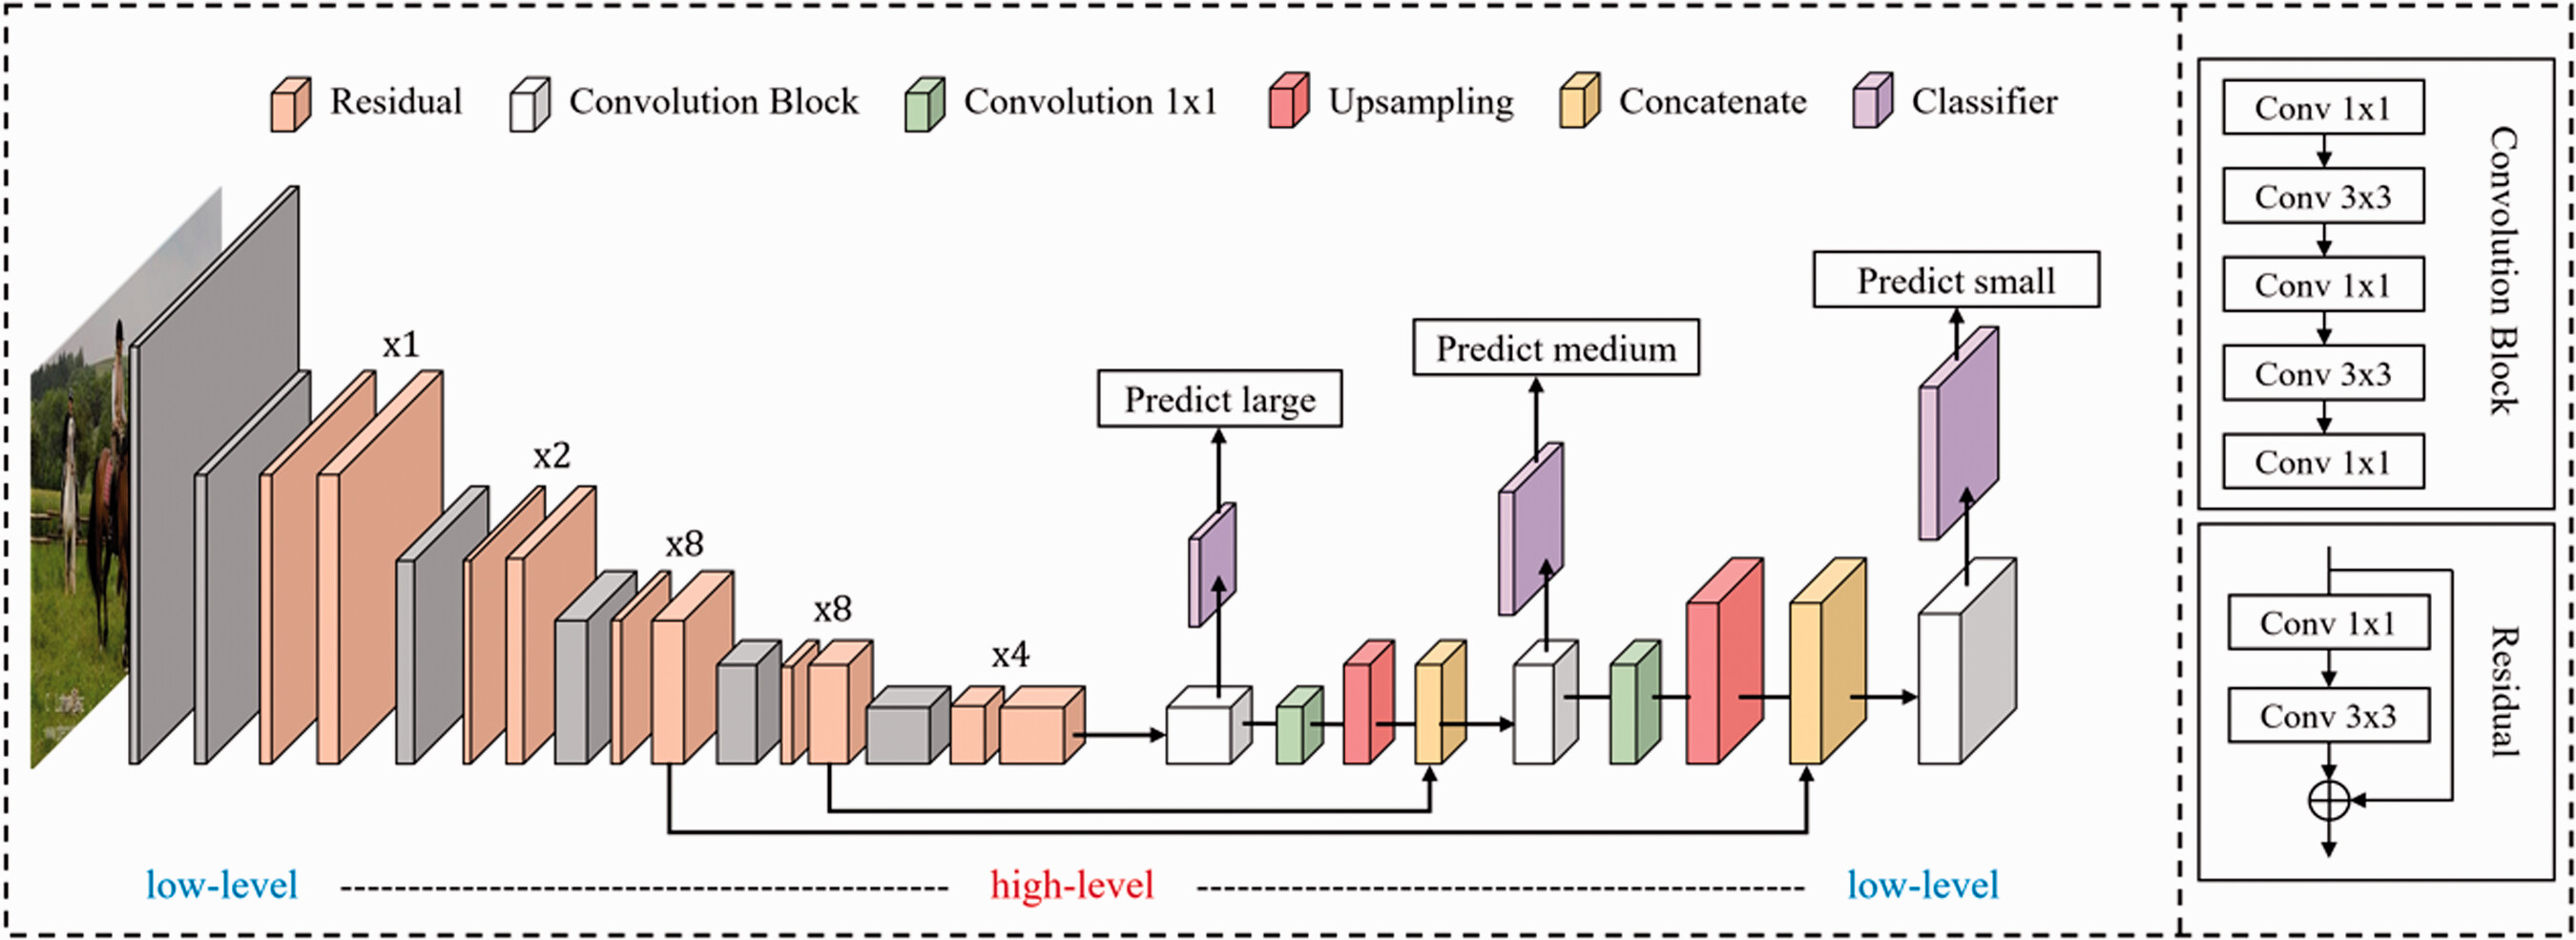
\includegraphics[width=16cm, height=5cm]{yolodos}
    \caption{Esquema de redes neuronales de YOLOv3.\protect\footnotemark}
    \label{fig:mesh1}
\end{figure}



\section{Objetivos y alcance}

\footnotetext{Imagen tomada de \url{https://journals.sagepub.com/cms/10.1177/0020720920983524/asset/images/large/10.1177_0020720920983524-fig2.jpeg}}

A continuación, se presentan los requisitos establecidos en la etapa de apertura del trabajo y su estado actual a la fecha. Es necesario tener en cuenta que, debido a cambios operativos, algunos de estos requisitos no pudieron ser cumplidos en su totalidad. \\ 

\begin{enumerate}
\item Requerimientos funcionales:
\begin{enumerate}
	\item El módulo debe detectar personas o animales de gran porte en áreas que el cliente defina como restringidas.
	\begin{itemize}
		\item Tipo: obligatorio
		\item Estado: finalizado
	\end{itemize}
	\item El módulo debe ser capaz de detectar a un intruso en un tiempo no mayor a 4 segundos.
	\begin{itemize}
		\item Tipo: obligatorio
		\item Estado: finalizado
	\end{itemize}
	\item El módulo debe correr en un computador de uso de hogar. Este debe ser comparable o menor a un Intel Core I5 y con no más de 8 GB de memoria RAM.
	\begin{itemize}
		\item Tipo: obligatorio
		\item Estado: finalizado
	\end{itemize}
	\item El sistema debe ser capaz de reconocer la presencia de intrusos, aun cuando el vídeo se haya registrado con el dron en movimiento.
	\begin{itemize}
		\item Tipo: obligatorio
		\item Estado: finalizado
	\end{itemize}
	\item \textbf{Requerimiento Opcional:} el sistema debe correr en un equipo que quepa a bordo de los drones (una Raspberry Pi, por ejemplo). 
	\begin{itemize}
		\item Tipo: opcional
		\item Estado: descartado
	\end{itemize}
\end{enumerate}
\item Requerimientos de documentación:
\begin{enumerate}
	\item El sistema deberá contar con un manual de usuario.
	\begin{itemize}
		\item Tipo: obligatorio
		\item Estado: finalizado
	\end{itemize}
	\item Se deberá contar con un manual de instalación del módulo desarrollado.
	\begin{itemize}
	 \item Tipo:obligatorio
	 \item Estado: finalizado
	\end{itemize}
	\item El código fuente deberá estar debidamente documentado.
	\begin{itemize}
		\item Tipo: obligatorio
		\item Estado : finalizado
	\end{itemize}
\end{enumerate}
\item Requerimientos de pruebas:
\begin{enumerate}
	\item El módulo deberá ser probado formalmente según indicaciones del cliente.
	\begin{itemize}
		\item Tipo: requisito modificado
		\item Estado: descartado
	\end{itemize}
	\item El cliente debe poder acceder en cualquier momento a la versión más reciente del código a través de GitHub.
	\begin{itemize}
	 \item Tipo: obligatorio
	 \item Estado: finalizado
	\end{itemize}
\end{enumerate}
\item Requerimientos de la interfaz:
\begin{enumerate}
	\item El usuario debe poder iniciar fácilmente la ejecución del módulo.
	\begin{itemize}
		\item Tipo: obligatorio
		\item Estado: finalizado
	\end{itemize}
\end{enumerate}
\item Requerimientos de interoperabilidad:
\begin{enumerate}
	\item \textbf{Opción A:} el módulo debe estar en capacidad de recibir el \textit{streaming} de vídeo de entre 4 y 8 drones.
	\begin{itemize}
		\item Tipo: requisito modificado
		\item Estado: descartado
	\end{itemize}
	\item \textbf{Opción B:} el módulo debe ser capaz de recibir un \textit{streaming} de vídeo y ejecutar la detección de intrusos en hardware dedicado a bordo.
	\begin{itemize}
		\item Tipo: requisito modificado
		\item Estado: descartado
	\end{itemize}
	\item Se requiere que el sistema pueda conectarse con otro módulo capaz de tomar decisiones con base en la información de detección de intrusos.
	\begin{itemize}
		\item Tipo: obligatorio
		\item Estado: finalizado
	\end{itemize}
\end{enumerate}
\end{enumerate}


A pesar de que algunos de los requerimientos funcionales fueron descartados dados algunos cambios que se presentaron en las plataformas del cliente, también hubo requerimientos que fueron agregados:

\begin{enumerate}
\setcounter{enumi}{5}
\item Requerimientos nuevos:
\begin{enumerate}
	\item El módulo deberá retransmitir los \textit{frames} procesados a un servidor indicado por el cliente. 
	\begin{itemize}
		\item Tipo: obligatorio
		\item Estado: finalizado
	\end{itemize}
\end{enumerate}
\end{enumerate}

Es importante tener en cuenta que el trabajo no contempló:

\begin{itemize}

	\item Reconocimiento del intruso: es decir, en caso de que se detecte a una persona, no se deberá dar con su identidad.
	
	\item Reacción del dron: es decir, una vez se haya detectado satisfactoriamente a un intruso, el sistema no deberá dar instrucciones específicas al dron, por ejemplo, de seguirlo.
	
	\item No existen requisitos específicos de cómo realizar la retransmisión de los \textit{frames} ya procesados.

\end{itemize}




\chapter{Introducción específica} % Main chapter title

\label{Chapter2}

%----------------------------------------------------------------------------------------
%	SECTION 1
%----------------------------------------------------------------------------------------
En este capítulo, se presentan los conceptos necesarios para poner en funcionamiento el trabajo de detección. Se inicia con la descripción de los objetos a detectar, seguido de los modelos de visión por computadora disponibles. De igual manera, se abordan los protocolos de transmisión y recepción del vídeo y se finaliza con los requerimientos computacionales necesarios para llevar a cabo la detección.

\section{Definición de intruso}
Para cumplir con el objetivo específico del trabajo, es importante tener en cuenta la definición de intruso dada por el cliente, que incluye la detección de personas y animales de gran porte, lo que implica que la respuesta del módulo deberá activarse con cualquier animal de mayor tamaño al de un perro o un gato. Es importante tener en mente que el \textit{dataset} COCO permite el reconocimiento de una serie de animales de gran porte que no hacen parte de la fauna argentina, por lo que se decidió en conjunto con el cliente que algunas etiquetas se filtrarían a fin de evitar que el modelo intente reconocer estas clases. Algunos ejemplos de etiquetas filtradas incluyen:

\begin{itemize}
	\item Elefantes
	\item Jirafas
	\item Cebras
\end{itemize}

Por otro lado, y a fin de mejorar el reconocimiento de intrusos, se decidió incorporar algunas clases que corresponden a objetos que suelen cargar las personas y vehículos. De esta manera se hace posible una suerte de reconocimiento indirecto, dándole al modelo una “segunda oportunidad” en casos en los que por algún motivo generó un falso negativo en el reconocimiento de una persona. Es importante tener en cuenta que estos objetos propuestos ya hacían parte del \textit{dataset} COCO, por lo que no se requirió reentrenar el modelo para lograr su detección. Dentro de estos objetos relacionados encontramos: 

\begin{itemize}
	\item Vehículos
	\item Objetos de porte personal, como maletines o sombrillas
\end{itemize}

Es importante tener en cuenta que el módulo marcará toda detección como una intrusión. Esto quiere decir que las detecciones en lotes vecinos no se filtrarán dado que se considera que la totalidad del \textit{frame} es área vigilada. Dicho esto, las clases que generarán un reporte positivo para intruso al ser detectadas son:

\begin{table}[]
\centering
\caption{Clases detectadas como intruso por el módulo.}
\label{definicion-intruso}
\begin{tabular}{cc}
\hline
\multicolumn{2}{c}{\textbf{Clases detectadas como intruso}} \\ \hline
Persona                   & Vaca                   \\
Camión                    & Bus                    \\
Automóvil                 & Sombrilla              \\
Motocicleta               & Mochila                \\
Bicicleta                 & Maletín                \\
Perro                     & Maleta                 \\
Caballo                   & Gato                   \\ \hline
\end{tabular}
\end{table}

\pagebreak

Hay que recordar que la sola detección de una de estas clases generará un reporte positivo de intruso. El modelo no está en capacidad de identificar personas específicas en el vídeo, por lo que le resultará imposible diferenciar entre personal autorizado en un área (el mismo personal de seguridad, o la persona al mando del dron), y a intrusos en la zona. 


\section{Modelo utilizado}

El modelo utilizado para el desarrollo de la totalidad del trabajo es YOLOv3. La principal ventaja que tiene este modelo es que es capaz de ejecutarse con una velocidad considerablemente mayor a la de modelos anteriores como RetinaNet-50 y RetinaNet-101. 

Este modelo se basa en el uso de redes neuronales convolucionales (CNN) que, al dividir la imagen en una cuadrícula, permiten calcular la probabilidad de ocurrencia de objetos en cada celda. Con esta información, el modelo determina tres parámetros clave para su funcionamiento:

\begin{itemize}
	\item \textit{Intersection over Union} (IoU) \cite{8}, se trata del criterio utilizado para eliminar cajas redundantes, y asegurar que solo se mantenga una por cada objeto detectado, incluso si hay varios objetos cercanos en la imagen. De esta manera, se evita la detección de objetos duplicados y se obtiene una detección más precisa y clara de los objetos presentes en la imagen.
	
	Se calcula a través de la ecuación \ref{eq:metric}:
	
\begin{equation}
	\label{eq:metric}
	IoU=\frac{A_{s}}{A_{u}}
\end{equation}
	
	
	
	Donde $A_{s}$ representa el área de superposición entre ambas cajas y $A_{u}$ el área de unión.
	
	Para lograr esto, cada celda es responsable de calcular la probabilidad de que haya un objeto dentro de sus fronteras, se genera una serie de cajas propuestas alrededor del objeto, y a través del uso de redes neuronales convolucionales se calcula la probabilidad de ocurrencia.
	
	Finalmente, el modelo elimina las cajas que no cumplen con dos criterios importantes:	en primer lugar, se descartan aquellas cajas que tienen una probabilidad de ocurrencia menor que la máxima del objeto de la zona. Este algoritmo es conocido como \textit{Non-Maximum Suppression} \cite{14} y utiliza la probabilidad de ocurrencia, también conocida como \textit{objectness score} \cite{12}, para seleccionar solo las cajas más relevantes. En segundo lugar, se eliminan las cajas que tienen un \textit{Intersection Over Union (IoU)} mayor a un valor determinado, que suele ser 0,45 aunque también se puede ajustar como parámetro en el modelo.
	
	
	\item \textit{Offset}: el \textit{offset} se refiere a la distancia medida desde la esquina superior izquierda de la celda con mayor probabilidad de contener un objeto \cite{10}. Esta medida es una forma eficiente de representar la posición de las cajas y reduce significativamente la cantidad de cálculos necesarios, lo que aumenta la eficiencia computacional del modelo \cite{9}. Una vez obtenido el \textit{offset}, se utilizan estos valores para calcular las coordenadas de las cajas que no fueron descartadas.
	\item Tensor: hace referencia a un vector utilizado para representar la probabilidad \cite{11} de que cada uno de los objetos incluidos en el \textit{dataset} COCO \cite{3} se encuentre en la caja . Esta representación no solo permite determinar la posición de diferentes objetos en la imagen, sino también discriminarlos por clases. La clase con mayor probabilidad es entonces reportada por el modelo.  
\end{itemize}

Es importante tener en cuenta que estos no son los parámetros finales arrojados por el modelo, sino que más adelante, la red calcula las coordenadas de la caja con la que se rodeará al objeto. Es decir, para cada objeto detectado, el modelo va a devolver (en ese orden):

\begin{itemize}
	\item pc: \textit{objectness score}, la probabilidad de que haya un objeto.
	\item bx: coordenada x del centro de la caja propuesta.
	\item by: coordenada y del centro de la caja propuesta.
	\item bh: altura de la caja propuesta.
	\item bw: ancho de la caja propuesta.
	\item c: tensor con la probabilidad de ocurrencia de las 80 clases que forman parte del \textit{dataset} COCO.
\end{itemize}


Esto se logra a través del uso de \textit{Anchor Boxes}: cajas de predicción predefinidas que el modelo va refinando a medida que analiza la imagen y calcula las métricas de cada uno de los objetos encontrados. A través de este método es posible eliminar la necesidad de una “ventana deslizante”, lo que a su vez permite analizar la totalidad de la imagen en un tiempo mucho menor que los métodos basados en aquel método, y, en consecuencia, se hace posible llevar a cabo un análisis en tiempo real. 

Dadas las bondades explicadas anteriormente, en conjunto con su facilidad de implementación en Python, se escogió partir del modelo YoloV3 y modificar su código fuente para lograr generar y extraer la información pertinente para completar el propósito del trabajo. Cabe aclarar que la decisión de utilizar este modelo se vio reforzada una vez se ejecutó la primera versión en tanto que el modelo está optimizado para funcionar con la tarjeta gráfica (NVIDIA Titan X), el código se pudo ejecutar satisfactoriamente, sin dejar a un lado los requisitos del trabajo en CPU (AMD Ryzen 5). 

\section{Protocolos de vídeo y transmisión}

El módulo del trabajo encargado de extraer y permitir el cálculo sobre cada uno de los \textit{frames} es OpenCV, por lo que los protocolos de vídeo aceptados corresponderán a los aceptados por OpenCV. En este sentido, el código está en capacidad de detectar intrusos en:

\begin{itemize}
	\item Vídeo guardado localmente
	\item Secuencia de imágenes
	\item URL de \textit{streaming} de vídeo
	\item \textit{Pipeline} Gstreamer
	\item Datos obtenidos desde \textit{webcam}
\end{itemize}

Sin embargo, es importante mencionar que, durante el desarrollo, se hicieron pruebas únicamente con los métodos de vídeo guardado localmente y URL de \textit{streaming} de vídeo. Los otros métodos no han sido probados, y, por lo tanto, no se podrá garantizar su correcto funcionamiento al solicitar al módulo ejecutarse utilizándolos como origen de datos. 

Por otro lado, y recordando que se trata de la biblioteca que hace posible extraer la información del vídeo para hacer posible su análisis, es de vital importancia tener en mente cuáles son los formatos de vídeo admitidos por OpenCV. Dentro de ellos se encuentran:

\begin{itemize}
	\item H264
	\item MPEG4
	\item AV1
\end{itemize}

Ahora bien, para acceder a ellos, bastará con pasar el link apropiado al método encargado. Dentro de los protocolos probados durante el desarrollo del trabajo se encuentran:

\begin{itemize}
	\item MQTT: es un protocolo que permite la comunicación entre dispositivos desarrollado por IBM. Este protocolo es considerado muy seguro debido a que utiliza un intermediario llamado MQTT Broker para el intercambio de información entre el servidor y el cliente. De esta forma, ninguna de las partes tiene acceso directo a los datos del otro, visto que solo cuentan con la información para acceder al MQTT Broker. En cambio, el cliente solicita una suscripción a un tema que le interesa (en este caso la transmisión de vídeo), y el agente se encarga de distribuir los mensajes enviados por el servidor. Está pensado especialmente para dispositivos IoT con recursos limitados y conexiones con poco ancho de banda. 
	\item RTMP: es un protocolo diseñado específicamente para la transmisión de audio y vídeo con gran rendimiento. Esto lo logra dividiendo la información en pequeños fragmentos, cuyo tamaño puede ser negociado de manera dinámica entre el cliente y el servidor de forma que la transmisión de vídeo se adapta mejor a las condiciones de la red de la que depende la transmisión. Sin embargo, dado que se trata de un protocolo diseñado para la transmisión de vídeo y audio con el menor \textit{delay} posible, este protocolo puede no ser el más adecuado cuando las condiciones de la red son limitadas. 
\end{itemize}

\section{Software y hardware utilizados} 

Para su funcionamiento, este trabajo requiere la presencia de algunos paquetes de software instalados en la máquina, los cuales son llamados directamente por el usuario cuando requiera la funcionalidad (por ejemplo, OBS Studio), o bien, que ya vienen incorporados en el código y por lo tanto, son un requisito indispensable para el trabajo y deberán encontrarse instalados. Dicho esto, es posible clasificar el software utilizado en tres categorías:


1. Paquetes de Python: son paquetes importados en el código a través del comando \textit{import}. Cabe mencionar que todos los paquetes son de código abierto. Ejemplos de estos paquetes son:
 
\begin{itemize}
	\item Numpy
	\item Matplotlib
	\item OpenCV
\end{itemize}
 
2. Código en Python: en especial para la implementación de la metodología YOLOV3. En internet está disponible el código fuente en formato Python (py).

3. Software completo: en particular para la retransmisión del vídeo procesado, se utilizó OBS Studio. Esta decisión responde a que, dentro del alcance del trabajo, no se definió ninguna actividad que no se encuentre directamente relacionada con la implementación de la detección de intrusos. Sin embargo, dado que se trata de un trabajo en el que se debe devolver la imagen procesada, es importante asegurarse que la retransmisión de los datos funcione de la manera correcta.

Más específicamente, las diferentes bibliotecas y paquetes de software utilizados para el desarrollo de este trabajo son:

% Please add the following required packages to your document preamble:
% \usepackage{graphicx}
\begin{table}[h]
\centering
\caption{Software requerido para el desarrollo y la ejecución del módulo.}
\label{software-requerido-mini}
\resizebox{\textwidth}{!}{%
\begin{tabular}{ll}
\toprule
\multicolumn{1}{l}{\textbf{Paquete}} & \multicolumn{1}{l}{\textbf{Función}}                       \\ \hline
PIP                         & Gestor de bibliotecas para Python                 \\
Numpy                       & Cálculos matriciales                              \\
OpenCV                      & Manipulación de imágenes y visión por computadora \\
Matplotlib                  & Creación de visualizaciones con Python            \\
Tensorflow                  & \textit{Framework} de machine learning                     \\
Pycharm                     & Ambiente de desarrollo                            \\
OBS Studio                  & \textit{Streaming} de vídeo                                \\
Python                      & Lenguaje en el que fue programado el módulo       \\
Ubuntu                      & Sistema operativo                                 \\ 
\bottomrule
\end{tabular}%
}
\end{table}

Es importante tener en cuenta que la totalidad de programas y bibliotecas utilizadas, tanto para el desarrollo, como para la ejecución del trabajo son software libre, por lo que no se requerirá adquirir ningún tipo de licencia para ponerlo en funcionamiento. En el apéndice \ref{AppendixA} se encuentra la tabla completa que incluye tipo de biblioteca, licencia y versión utilizada.

De igual manera, cabe resaltar que OBS Studio es el programa de retransmisión elegido teniendo en cuenta que esta es una característica que se encuentra fuera del alcance del trabajo y por lo tanto, cuya implementación es necesaria a través de este método mientras que hacerlo a través de software integrado en el código fuente (como FFMpeg) será parte del alcance de trabajos posteriores. 

El paquete de Python ya viene instalado por defecto en la instalación de Ubuntu, por lo que no se requerirá su instalación. El resto de los paquetes, sin embargo, deberán ser instalados de acuerdo con el manual de instalación que se entrega al cliente, en el que se detalla de manera minuciosa cuál es el procedimiento que se debe seguir a fin de instalar correctamente todos los paquetes. 

De igual manera, se debe tener en cuenta que dadas las restricciones de la máquina en la que se desarrolló el trabajo, la totalidad del desarrollo fue llevado a cabo en máquinas virtuales a través del uso de programas de virtualización como VMware Workstation \cite{7}. 
Dentro de los requerimientos mínimos de hardware del trabajo, se tienen los siguientes:

\begin{itemize}

	\item Procesador: AMD Ryzen 5
	\item Tarjeta gráfica: no requerida
	\item Memoria RAM: 6 GB. 

\end{itemize}

Es importante tener en cuenta que los listados anteriormente son los requisitos mínimos del sistema, que van a garantizar que el trabajo se ejecute cumpliendo con los requerimientos del cliente. Sin embargo, se recomiendan las siguientes características del sistema para un rendimiento óptimo a la hora de ejecutar el módulo.

\begin{itemize}

	\item Procesador: Intel Core i7
	\item Tarjeta gráfica: NVidia Tesla T4 o NVidia Titan X.
	\item Memoria RAM: 8 GB. 

\end{itemize}

El modelo YoloV3, sobre el que está basado el desarrollo del trabajo utiliza de manera extensiva la API Cuda de NVIDIA. Por este motivo, tratar de ejecutar el módulo en tarjetas gráficas de AMD resultará en el modelo siendo llevado al procesador por Tensorflow. En consecuencia, se afirmará que el trabajo resulta incompatible con estas tarjetas gráficas. Esto fue comprobado con el uso de una tarjeta AMD Radeon Vega 8.  
\chapter{Diseño e implementación} % Main chapter title

\label{Chapter3} % Change X to a consecutive number; for referencing this chapter elsewhere, use \ref{ChapterX}

\definecolor{mygreen}{rgb}{0,0.6,0}
\definecolor{mygray}{rgb}{0.5,0.5,0.5}
\definecolor{mymauve}{rgb}{0.58,0,0.82}

%%%%%%%%%%%%%%%%%%%%%%%%%%%%%%%%%%%%%%%%%%%%%%%%%%%%%%%%%%%%%%%%%%%%%%%%%%%%%
% parámetros para configurar el formato del código en los entornos lstlisting
%%%%%%%%%%%%%%%%%%%%%%%%%%%%%%%%%%%%%%%%%%%%%%%%%%%%%%%%%%%%%%%%%%%%%%%%%%%%%
\lstset{ %
  backgroundcolor=\color{white},   % choose the background color; you must add \usepackage{color} or \usepackage{xcolor}
  basicstyle=\footnotesize,        % the size of the fonts that are used for the code
  breakatwhitespace=false,         % sets if automatic breaks should only happen at whitespace
  breaklines=true,                 % sets automatic line breaking
  captionpos=b,                    % sets the caption-position to bottom
  commentstyle=\color{mygreen},    % comment style
  deletekeywords={...},            % if you want to delete keywords from the given language
  %escapeinside={\%*}{*)},          % if you want to add LaTeX within your code
  %extendedchars=true,              % lets you use non-ASCII characters; for 8-bits encodings only, does not work with UTF-8
  %frame=single,	                % adds a frame around the code
  keepspaces=true,                 % keeps spaces in text, useful for keeping indentation of code (possibly needs columns=flexible)
  keywordstyle=\color{blue},       % keyword style
  language=[ANSI]C,                % the language of the code
  %otherkeywords={*,...},           % if you want to add more keywords to the set
  numbers=left,                    % where to put the line-numbers; possible values are (none, left, right)
  numbersep=5pt,                   % how far the line-numbers are from the code
  numberstyle=\tiny\color{mygray}, % the style that is used for the line-numbers
  rulecolor=\color{black},         % if not set, the frame-color may be changed on line-breaks within not-black text (e.g. comments (green here))
  showspaces=false,                % show spaces everywhere adding particular underscores; it overrides 'showstringspaces'
  showstringspaces=false,          % underline spaces within strings only
  showtabs=false,                  % show tabs within strings adding particular underscores
  stepnumber=1,                    % the step between two line-numbers. If it's 1, each line will be numbered
  stringstyle=\color{mymauve},     % string literal style
  tabsize=2,	                   % sets default tabsize to 2 spaces
  title=\lstname,                  % show the filename of files included with \lstinputlisting; also try caption instead of title
  morecomment=[s]{/*}{*/}
}


%----------------------------------------------------------------------------------------
%	SECTION 1
%----------------------------------------------------------------------------------------
En este capítulo se detallan los aspectos técnicos del desarrollo del trabajo. Incluye las consideraciones tomadas en cuenta durante el desarrollo, el detalle de las modificaciones realizadas al modelo de partida, así como el detalle del papel que juega el módulo en el sistema. De igual manera, se hace una descripción cronológica del desarrollo del módulo.    

\section{Consideraciones generales}

El módulo de inteligencia artificial propuesto es una implementación del modelo YOLOv3, especialmente modificada para cumplir con las necesidades específicas del cliente, así como una serie de requisitos funcionales.  Es por esto que fue necesario hacer modificaciones a los archivos originales de la biblioteca. 

Como se puede observar en el capítulo 1, no todos los requerimientos funcionales propuestos para el inicio del trabajo pudieron ser cubiertos. Recordando que esta versión del trabajo representa un mínimo producto viable, a continuación se presenta una lista de todos los requerimientos funcionales que fueron cubiertos:

\begin{itemize}

	\item El módulo se ejecuta en un computador de uso de hogar. 
	\item El módulo es capaz de reconocer 14 clases como intruso. 
	\item Se reporta al usuario de manera visual. 
	\item Se reporta al usuario a través de un archivo de fácil análisis.
	\item Resulta muy sencillo iniciar la ejecución del módulo a través de su interfaz grafica. 

\end{itemize}

De igual manera, el módulo está construido de manera que realizar modificaciones, o bien, expandir su funcionalidad en un futuro resulte muy sencillo. Es de vital importancia recalcar que esto se hizo teniendo en cuenta que se trata de un módulo que, a fin de salir de este estatus de mínimo producto viable, deberá sufrir un proceso de optimizacion muy fuerte. Algunos ejemplos de puntos en los que se pueden aplicar estos trabajos son:

\begin{itemize}

	\item El módulo está diseñado para filtrar las etiquetas que no hacen parte de las clases dadas en la definición de intruso. Esto implica que, a pesar de que no se reporte en ninguna de las dos metodologías, el módulo aún reconoce otras clases. En otras palabras, si se puede observar un modelo en el \textit{frame}, este será satisfactoriamente detectado y son los métodos encargados del reporte los que no lo entregarán como un resultado positivo. 
	\item La precisión del modelo debe ser mejorada: dado que ocasionalmente se hacen detecciones de objetos que no corresponden con lo visto en el \textit{frame}. Se detectó que, en particular, el módulo es especialmente susceptible a generar falsos positivos. 
	\item Los cuadros se devuelven en espacio de color bgr. Esto, en combinación con que el color de los rectángulos no se puede cambiar desde la interfaz grafica.
	\item El color de los rectángulos es igual para todas las clases de objeto.
	\item Se debe mejorar significativamente el manejo que da el módulo de las excepciones que se generen, tanto a nivel de manejo de problemas originados en el código mismo, como recuperación cuando se generen cortes en la recepcion del \textit{streaming} de video.
	\item A pesar de que la interfaz grafica se realizó pensando en la facilidad de uso para el usuario, su comportamiento podría resultar extraño dado que el diseño de experiencia de usuario (UX) quedó fuera del alcance de los trabajos durante su etapa de concepción. 

\end{itemize}

Finalmente, resulta de especial interés tener en mente también las limitaciones del modelo:

\begin{itemize}

	\item Los modelos YOLO se ven limitados cuando se les pide detectar objetos que se encuentran muy cerca de una fuente de luz muy brillante, especialmente el sol, se pueden generar dificultades para detectar los objetos. Esto es parcialmente contrarrestado añadiendo las clases adicionales detalladas en la tabla \ref{clases-auxiliares-etiquetas}. 
	\item Los objetos deben encontrarse a una distancia prudencial del dron. A pesar de que las pruebas de vuelo no se han enfocado en el cálculo de este valor, sí se hace evidente que al estar el dron demasiado lejos de ellas, no se hace una detección oportuna. 
	\item El modelo no cuenta con funciones de \textit{auto-healing}, que deberían ser tenidas en cuenta a fin de lograr mantener la integridad del modelo si sus pesos son actualizados constantemente por el cliente a fin de mejorar la predicción. 

\end{itemize}

\section{Arquitectura del módulo}

Se propone como mínimo producto viable de este módulo, un código altamente modular. Esto significa que la manera en la que está desarrollado (a excepción del método principal, en el archivo Utils), está planteada en pequeños métodos que podrán ser modificados y mantenidos con facilidad. Esto supone, sin embargo, que sea de vital importancia entender la arquitectura del módulo a fin de poder realizar las modificaciones pertinentes en el punto adecuado del código. Así como se hizo en el numeral anterior (consideraciones generales) con el flujo de información entre el sistema y el módulo, a continuación, se describe el flujo de la información en el interior del módulo.   

El módulo está compuesto por cuatro capas funcionales:

\begin{enumerate}

	\item Funciones originales de YOLO: encargadas de la funcionalidad base de detección de los objetos en la totalidad de las clases que componen el \textit{dataset} COCO. Incluye funciones como nms (encargada del \textit{non-max supression}) y la función IoU. 
	\item Funciones híbridas: normalmente funciones que coordinan el llamado de las demás funciones. A pesar de que ofrecen una funcionalidad muy similar a las originales de YOLO, funcionan en un orden diferente, de forma que se puedan obtener los datos requeridos en el momento preciso para las necesidades del cliente.  
	\item Funciones propias: que permiten agregar al módulo la funcionalidad requerida por el cliente. Ejemplos de estas funciones incluyen la generación de archivos en formato CSV y la carga de etiquetas válidas. 
	\item Interfaz gráfica: que permite al usuario interactuar con el módulo para iniciar su ejecución fácilmente. 

\end{enumerate}

El diagrama de bloques correspondiente a estas cuatro capas es el siguiente:

\begin{figure}[!ht]
    \centering
    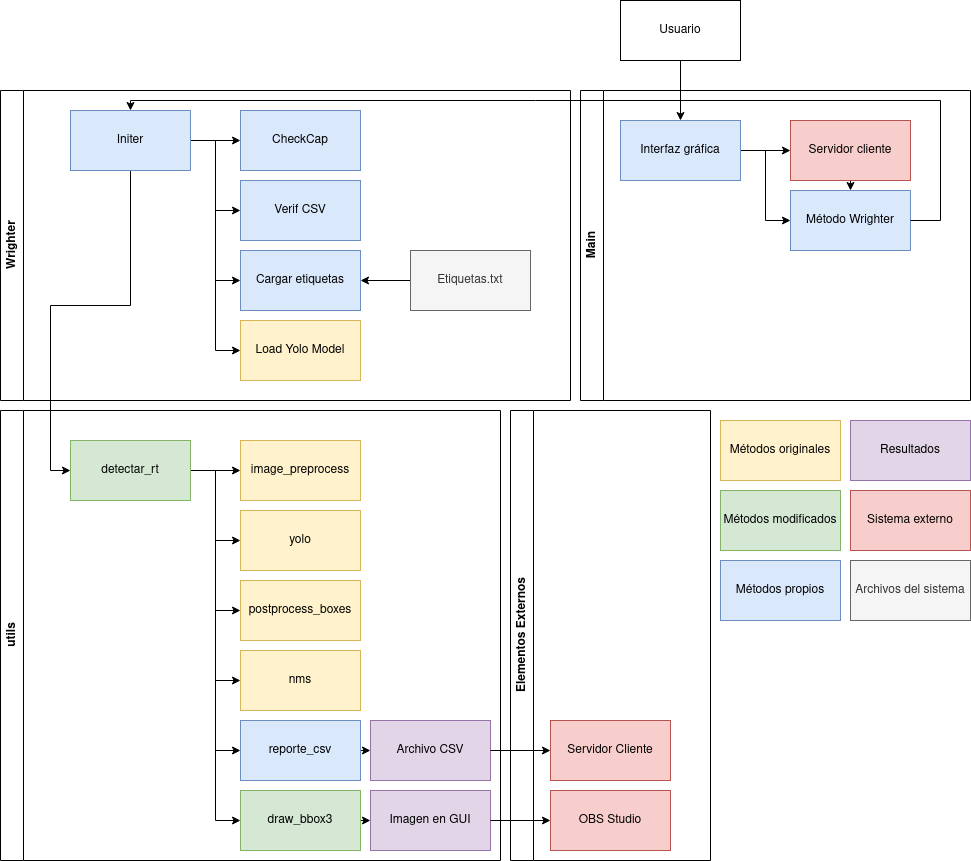
\includegraphics[width=16cm, height=14cm]{c31v2}
    \caption{Diagrama de bloques del módulo.}
    \label{fig:mesh1}
\end{figure}


\section{Esquema detallado del módulo en el interior del sistema}

Este módulo es una parte de un trabajo más grande desarrollado directamente por el cliente. Es decir, deberá estar en capacidad de comunicarse con otras partes del sistema, de forma que estos otros módulos puedan tomar decisiones y recibir órdenes de controladores humanos. A pesar de que se desconoce el funcionamiento de la totalidad del sistema.  

Para lograr esto, durante la fase de concepción del trabajo se estipuló que el módulo deberá ser capaz de conectarse a los servidores del cliente, en los que se aloja la transmisión de vídeo. Esta conexión entre ambos equipos se logra cuando el usuario indica al módulo, a través de la interfaz gráfica (visible en la imagen). Una vez se presiona el botón “Iniciar ejecución”. Esta interfaz está pensada para ser tan sencilla como sea posible, permitiendo que el usuario inicie la ejecución del módulo de la manera más sencilla posible.

\begin{figure}[!ht]
    \centering
    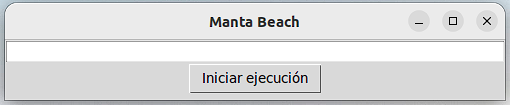
\includegraphics[width=10cm, height=2cm]{c32}
    \caption{Interfaz gráfica del módulo.}
    \label{fig:gui}
\end{figure} 

Por otro lado, el módulo deberá reportar al resto del sistema si se detectó a algún intruso. Para esto, se definieron dos metodologías, que se detallarán más adelante en este capítulo:

\begin{enumerate}

	\item Reporte visual
	\item Reporte en formato CSV

\end{enumerate}

Dada esta descripción, desde afuera, el módulo tendrá el siguiente aspecto:

\begin{figure}[!ht]
    \centering
    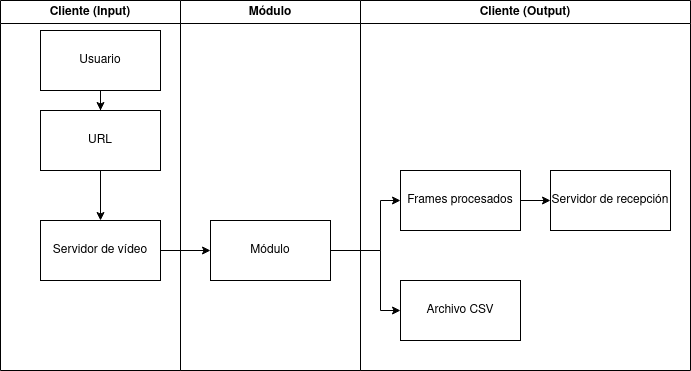
\includegraphics[width=16cm, height=9cm]{c33v2}
    \caption{Diagrama de bloques del módulo en el interior del sistema.}
    \label{fig:mesh1}
\end{figure} 

Cabe mencionar que, dada la naturaleza confidencial de este módulo, así como de la totalidad del sistema, se buscó que el módulo requiriera la menor cantidad de información para funcionar como fuese posible. Esto también permite que los parámetros dados del vídeo y la cantidad de transmisiones que se procesan a la vez se encuentren bajo total control del cliente. 

De igual manera es de vital importancia tener en cuenta que la totalidad del módulo se desarrolló sin conocer el funcionamiento del resto del sistema. Es por esto que para iniciar su ejecución se debe ejecutar el código de manera manual. El sistema no puede detectar cuándo se ha iniciado una transmisión, y por lo tanto, se requiere de una persona encargada de dar inicio cuando sea necesario. 

Finalmente, este módulo está diseñado como un mínimo producto viable que permita a las personas tomar decisiones informadas, con soporte en vídeo. Esta versión no se considera un sistema autónomo, sino que constituye un sistema de apoyo a la decisión. 


\section{Esquema detallado de las modificaciones hechas al modelo}

Dado que se trata de una implementación personalizada, existen varias diferencias entre el módulo desarrollado y la implementación original del modelo YOLOv3. Dicho esto, las modificaciones realizadas generales al modelo, en orden cronológico son las siguientes:

\begin{itemize}

	\item Se preparó el código para que se ejecute desde un \textit{streaming} de vídeo, en vez de un archivo local en el equipo. Esto implica que se debe detener la ejecución antes de pasar imágenes al método de detección si no es posible establecer conexión con el servidor.
	\item Se filtraron las etiquetas a fin de lograr que solo sean detectadas las clases definidas en la definición de intruso.
	\item Se crearon los métodos encargados de generar una respuesta que se pasará al resto del módulo. Particularmente, se le permitió al programa generar dos tipos de respuesta.
	\item Se estableció un método que permite descartar un número determinado de \textit{frames}, de forma que se permita aliviar la carga computacional sobre el equipo.
	\item Durante el desarrollo del módulo se estableció que el hacer que el módulo sea capaz de procesar varios \textit{streamings} de vídeo de manera paralela está fuera del alcance de las temáticas cubiertas en el postgrado, a fin de cubrir satisfactoriamente este requisito, se informó al cliente que sería posible este análisis en caso de que se reciba el \textit{streaming} con varias cámaras combinadas en un único cuadro. Esto, por ser una decisión relacionada con la forma en la que el cliente maneja su \textit{streaming}, no afectó el desarrollo del trabajo. 

\end{itemize}

Cabe resaltar que cada una de estas modificaciones implicó una serie de tareas más pequeñas, a las que Manta Beach, como cliente, hizo un seguimiento cercano.

\section{Ajustes para cumplir con el rendimiento requerido}

Dadas las limitantes del equipo en el que se realizó el desarrollo del módulo (especialmente teniendo en cuenta que este desarrollo se hizo utilizando máquinas virtuales), fue necesario llevar a cabo un análisis detallado que, en teniendo en mente las necesidades del cliente, permitiera reducir la carga computacional sobre la máquina. De esta manera se intentó una serie de ajustes al modelo de forma que se lograra mantener los requisitos dados en el proceso de establecimiento de los trabajos:

\begin{itemize}
 	\item Eliminación de un número determinado de \textit{frames}. Si bien, este es un número fácil de establecer, y que el sistema recibirá como parámetro, se recomienda utilizar un valor de N=10, de forma que, para un fps de 30, se analicen 3 cuadros por segundo. Cabe resaltar que 30 será el número máximo para cumplir con el requisito de hacer un análisis en un tiempo no mayor a 1 segundo, mientras que con N=120, se cumplirá el requisito de hacer un análisis en un tiempo no mayor a 4 segundos.
 	\item Reducción de la calidad del \textit{streaming} de vídeo a 200. A pesar de que esta reducción afecta muy notoriamente la calidad del vídeo, el módulo es capaz de detectar objetos. Se pierden, sin embargo, las propiedades probatorias del trabajo. En la imagen se puede ver un ejemplo del vídeo con calidad reducida. Como se mencionó en secciones anteriores este es un parámetro qué el módulo ya recibe en el \textit{streaming} de vídeo, y cuyo control recae únicamente en el cliente. 
 
\end{itemize}

Finalmente, la solución escogida fue descartar uno de cada N \textit{frames}, de forma que no se procese la totalidad de ellos, y se requiera una mejor cantidad de operaciones. Cabe mencionar que, en este tipo de modelos, es común que conforme se aumente el rendimiento, también se reducirá la precisión del modelo. Es por esto que, para contrarrestar estos efectos, se decidió incluir algunas clases que permitieran hacer una detección indirecta. Estas clases corresponden a objetos que las personas cargan con frecuencia. Estas clases adicionales son: 

\begin{table}[h]
\centering
\caption{Clases auxiliares para detección indirecta.}
\label{clases-auxiliares-etiquetas}
\begin{tabular}{cc}
\hline
\multicolumn{2}{c}{\textbf{Clases auxiliares}} \\ \hline
Camión                	  & Bicicleta              \\
Automóvil                 & Bus		               \\
Motocicleta               & Sombrilla              \\
Mochila			          & Maletín                \\  \hline
\end{tabular}
\end{table}

Por la naturaleza del trabajo, cabe aclarar, en este punto, que el módulo no podrá discernir que al detectar simultáneamente la clase mochila y la clase persona en un espacio muy cercano, podrá tratarse de una única detección. Estas serán registradas y reportadas por el módulo como dos detecciones separadas. 

Esto, sin embargo, es preferible a eliminar detecciones, teniendo en mente que se prefiere que el módulo pueda detectar a tantas personas como sea posible, dada la sensibilidad de las consecuencias en caso de una falla del modelo. 

\section{Entrega de resultados obtenidos al resto del software y retransmisión del vídeo procesado}

Una vez que se ha analizado el \textit{frame}, el módulo deberá ser capaz de devolver resultados al resto del sistema, de forma que tanto las personas encargadas, como el sistema mismo sean capaces de tomar decisiones rápidas, e informar cómo proceder. Dados estos dos actores a los que se les debe hacer llegar la información, en conjunto con el cliente se decidieron utilizar dos métodos diferentes a través de los que el módulo dará su respuesta para cada uno de los \textit{frames}:

\begin{itemize}

	\item Entrega visual: imagen procesada con sus cajas identificando los objetos detectados. Estos \textit{frames} ya procesados son retransmitidos al servidor original para su visualización en la plataforma designada por el cliente. Es importante tener en cuenta que, en esta versión del módulo, esta retransmisión no se hace directamente a través del módulo propuesto, sino que se requerirá el uso de software externo, como el OBS Studio. 
	\item Entrega para análisis de datos: archivo en formato CSV con la información de los objetos detectados. De igual manera, el sistema será capaz de reportar el número del dron desde el que se hizo la detección, a pesar de que es una característica que no se ha probado, teniendo en cuenta que aún no se han hecho vuelos con varios drones de manera simultánea. A diferencia de la imagen preprocesada, este archivo no es retransmitido. Se guarda por defecto en la carpeta de documentos de la máquina en la que se está ejecutando. Visto que esta versión corresponde a un mínimo producto viable, este archivo no se retransmite. Se guarda, en cambio, en la carpeta de documentos de la máquina en la que se ejecuta el módulo. 

\end{itemize}

Es muy importante tener en mente que se espera que no haya personas supervisando constantemente las cámaras. Por este motivo, es posible deshabilitar la retransmisión del \textit{frame} procesado. Por otro lado, y buscando que el sistema sea tan autónomo como resulte posible, no se podrá desactivar el reporte a través de archivos CSV.

\begin{figure}[!ht]
    \centering
    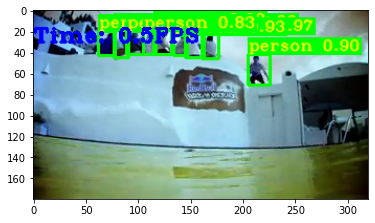
\includegraphics[width=8cm, height=5cm]{sampleGrecia}
    \caption{Ejemplo de resultados generados por el módulo.}
    \label{fig:grecia}
\end{figure}



Por otro lado, los archivos CSV deberán contener los siguientes datos:

\begin{itemize}
	\item Fecha y hora de detección.
	\item Coordenadas de detección dentro del \textit{frame}.
	\item Número de dron en el que ocurre la detección.
\end{itemize}

Los datos serán entregados en el orden en el que han sido mencionados. Esto es de vital importancia de forma que el resto del sistema sea capaz de interpretar correctamente los datos entregados. Por otro lado, se debe recordar que el sistema desconoce la ubicación del dron en su recorrido de vuelo. Es por esto que el módulo no podrá reportar la ubicación en la que detectó el objeto. Esta deberá ser calculada por el sistema a partir de los datos de posición, altura y posición en el \textit{frame} (información proporcionada por el módulo).
% Chapter Template

\chapter{Ensayos y resultados} % Main chapter title

\label{Chapter4} % Change X to a consecutive number; for referencing this chapter elsewhere, use \ref{ChapterX}

%----------------------------------------------------------------------------------------
%	SECTION 1
%----------------------------------------------------------------------------------------
Este capítulo detalla las distintas pruebas que se hicieron sobre el módulo, así como el proceso de descarte de módulos a bordo de los drones. De igual manera, detalla los resultados obtenidos durante estos ensayos y los criterios utilizados para dar por cerrados los distintos requerimientos presentados en el capítulo 1. Finalmente, se explican los resultados mostrados durante una ejecución exitosa del módulo. 

\section{Descripción del proceso de pruebas}
%\label{sec:pruebasHW}

A pesar de que esto se estipuló en la concepción inicial del trabajo, conforme se dio su avance no se hizo posible llevar a cabo un proceso formal de pruebas al módulo. Sin embargo, el cliente estuvo involucrado directamente en el proceso de verificación de la funcionalidad del módulo a través de reuniones quincenales.

En estas reuniones fue posible hacer un seguimiento muy cercano y dar aprobación a las siguientes características para el funcionamiento del módulo. Durante estas reuniones se hizo posible dar por aprobado el código presentado para el trabajo, teniendo en cuenta que se cumplió con los siguientes criterios:

\begin{itemize}

	\item El módulo obtiene correctamente los \textit{frames} enviados por el cliente en el servidor que este dispone para tal fin.
	\item El módulo detecta intrusos en un tiempo no mayor a 4 segundos, aún cuando se ejecute en sistemas considerablemente menores a los que se espera lo ejecuten. En particular, utilizando CPU en vez de GPU durante la detección.
	\item La precisión del modelo es razonable.
	\item Fue posible hacer la detección en tiempo real. Es decir, no solo se ejecutó con vídeos de prueba grabados por el cliente, sino que el módulo también se ejecutó correctamente durante vuelos transmitidos en tiempo real.
	\item El módulo es capaz de detectar intrusos en varios \textit{streamings} de vídeo. Se deja la anotación que para que esto se logre, se deberá preprocesar el vídeo de forma que todos los \textit{streamings} vengan combinados en un único \textit{frame}. El módulo no tiene la capacidad de ejecutar varias instancias de manera paralela. 
	\item Se realizó una serie de pruebas durante estas reuniones, en las que se evidenció el funcionamiento del módulo. 

\end{itemize}

Para este visto bueno, no fueron considerados los siguientes requisitos, a pesar de que se trata de tareas que fueron ejecutadas:

\begin{itemize}
	\item Documentación del módulo.
	\item Facilidad de uso del módulo.
	\item Sistema operativo en el que se ejecutará el módulo. A pesar de que, durante la etapa de planificación, no se especificó el sistema operativo en el que se ejecutará el modelo, este fue diseñado para ejecutarse en Ubuntu 22.04. 
\end{itemize}

\section{Pruebas en Raspberry Pi}

Desde la concepción inicial del trabajo, se estableció que se tendrían dos caminos para poder desarrollarlo: por un lado, se planteó que el módulo debía ser capaz de reconocer intrusos en varios \textit{streamings} de vídeo simultáneos (camino que finalmente se vio favorecido), o bien, hacer que el módulo fuese capaz de correr en equipos a bordo de los drones. Para esto, se llevaron a cabo una serie de pruebas y ensayos en equipos Raspberry Pi. Más concretamente, las especificaciones de los equipos sobre los que se hicieron las pruebas son:

\begin{itemize}
	\item Modelo: Raspberry Pi 2 modelo B
	\item Sistema operativo: Raspberry Pi OS (Debian 11 – Bullseye)
	\item CPU quad-core ARM Cortex-A7 900MHz
	\item Memoria ram: 1 Gb.
	\item Overclocking: Desactivado

\end{itemize}

Específicamente, el modelo con el que se tuvo los problemas más importantes a la hora de la instalación fue la versión completa de Tensorflow, requerida para la ejecución del módulo. Cabe mencionar que las placas Raspberry Pi son compatibles con la versión Lite de Tensorflow. Dicho esto, se intentaron cinco métodos para la instalación de esta biblioteca. Ninguno de ellos fue exitoso. El proceso llevado a cabo en cada una de las cinco instalaciones fue el siguiente:

\begin{itemize}
 \item Instalación 1 \cite{16}:
 	\begin{itemize}
 
 		\item instalación de Tensorflow: utilizando PIP.
 		\item se clona el repositorio de GIT de Tensorflow.
 	
 	\end{itemize}
 \item Instalación 2 \cite{17}:
 	\begin{itemize}
 		\item instalación de Tensorflow: utilizando PIP y el comando –no-cache-dir.
 	\end{itemize}
 \item Instalación 3 \cite{19}:
 	\begin{itemize}
 		\item instalación de Tensorflow Lite: utilizando PIP.
 	\end{itemize}
 \item Instalación 4 \cite{18}:
 	\begin{itemize}
		\item instalación de Libatlas: utilizando PIP.
 		\item instalación de Tensorflow: utilizando PIP.
 	\end{itemize}
 \item Instalación 5 \cite{20}:
 	\begin{itemize}
 		\item Descarga de los paquetes y llaves disponibles en:
 			\begin{itemize} 
 				\item https://packages.cloud.google.com/apt
 				\item https://packages.cloud.google.com/apt/doc/apt-key.gpg
 			\end{itemize}
 		\item Se agregaron estos paquetes y llaves a Debian.
 		\item Instalación de Libatlas: usando PIP.
 		\item Instalación de Tensorflow: usando PIP.
 	\end{itemize}
\end{itemize}


Al tratar de importar esta biblioteca en el código de Python, se obtuvo un fallo en todas las instancias, por lo que se decidió no continuar con esta aproximación para dar solución a la problemática. Es importante destacar que, dado que el módulo se desarrolló tomando como base el modelo YOLOv3 original (no el modelo Lite), no se cumplía con las especificaciones requeridas por este tipo de equipos, y una segunda implementación del modelo utilizando la versión YOLOv3 Lite hubiese implicado en sí, el trabajo equivalente a un módulo completo adicional.

De igual manera atrae particular atención mencionar que la placa con la que se contaba era un modelo antiguo de Raspberry Pi (Raspberry Pi 2 Modelo B de febrero de 2015), que no cuenta con una compatibilidad tan completa como la que se da con una Raspberry Pi 4. Es, entonces, muy importante considerar placas más avanzadas, como la Raspberry 4, en caso de que se decida continuar con el desarrollo de módulos a bordo de los drones.  


\section{Caso de Uso}

Una vez establecido el funcionamiento interno del módulo, se hace importante también tener en cuenta el flujo de trabajo para iniciarlo y ponerlo en funcionamiento. Se contemplar las siguientes consideraciones para que se pueda iniciar el módulo de la manera correcta:

\begin{itemize}

	\item Se debe contar con los links a los servidores de transmisión y recepción.
	\item El servidor de conexión debe estar transmitiendo.
	\item Se debe contar con la llave de transmisión proporcionada por el cliente.

\end{itemize}

En total, se debe seguir n pasos (contando el paso 0 de inicio de sesión en el sistema operativo y 1 de instalación) para lograr el funcionamiento esperado del módulo:

\begin{enumerate}
	\item El usuario deberá iniciar sesión en Ubuntu 22.04 LTS. Deberá cerciorarse que lo haga utilizando xorg. A pesar de que esta versión Ubuntu es compatible con el gestor de ventanas Wayland, su uso podrá causar una ejecución inestable del módulo. 
	\item Instalación del módulo: este paso contempla la instalación del módulo en una instalación nueva de Ubuntu 22.04 LTS. Para esto, el usuario se deberá remitir al manual de instalación que se entregó al cliente. Como esta versión no cuenta con una versión empaquetada en formato .deb (compatible con los sistemas basados en Debian), este paso incluirá la descarga de un IDE y la correspondiente apertura del código fuente.
	\item Ejecutar el código fuente en el archivo Main. Esto permitirá la apertura de la interfaz gráfica (visible en la figura \ref{fig:gui}). Aquí el usuario podrá introducir el link proporcionado por el cliente.
	\item En el caso de una conexión exitosa al servidor de transmisión, el usuario verá que aparecerá una ventana en su pantalla mostrando los \textit{frames} procesados por el módulo. Este no fue uno de los requisitos expuestos en la etapa de planificación del proyecto: fue agregado posteriormente durante el desarrollo del trabajo.  
	\item El usuario encontrará en su carpeta de documentos el archivo CSV con todas las detecciones de la fecha.
	\item A fin de retransmitir los \textit{frames} procesados de regreso a los servidores del cliente, el usuario deberá abrir OBS Studio de manera independiente. Dentro de este programa, el usuario deberá seguir los siguientes pasos:
	\begin{enumerate}
		\item Crear un nuevo origen de datos, que corresponderá a la ventana generada por el módulo (mencionada el paso 3).
		\item Dirigirse a las configuraciones de OBS Studio, particularmente en la pestaña \textit{Stream}.
		\item Proporcionar el link de \textit{streaming} y su respectiva llave de transmisión.
	\end{enumerate}
	\item Observar el \textit{streaming} en el visor que el cliente disponga para este fin. 
\end{enumerate}

De igual manera, una vez logrado esto, es importante observar los resultados obtenidos durante la ejecución del módulo: 

\begin{itemize}
	\item El módulo se ejecutó con un promedio de 0,54 fps. Este valor es mayor al requisito del cliente de procesar un número mayor a 0,25 fps. Estos valores se lograron con CPU, ejecutados en una máquina virtual.
	\item En promedio se pierden en la transmisión, un 15\% de los \textit{frames}. Si bien, el módulo los reporta (según la imagen \ref{fig:grecia}), es capaz de recuperarse satisfactoriamente de esta situación.
	\item El modelo requiere un breve período de calentamiento para lograr las métricas mencionadas arriba. En este momento los fps son menores a los que logrará el modelo en su ejecución normal. 

\end{itemize} 
% Chapter Template

\chapter{Conclusiones} % Main chapter title

\label{Chapter5} % Change X to a consecutive number; for referencing this chapter elsewhere, use \ref{ChapterX}


%----------------------------------------------------------------------------------------

%----------------------------------------------------------------------------------------
%	SECTION 1
%----------------------------------------------------------------------------------------

En este capítulo se detallan los resultados obtenidos del proceso del desarrollo del módulo. Es decir, se hace un recuento de las características finales del mínimo producto viable que resultó de este proceso sin detallar ejecuciones específicas. 

\section{Resultados Obtenidos}
Del desarrollo del modelo surgieron una serie de conclusiones que representan, o bien, trabajos futuros (detallados en secciones posteriores), o recomendaciones para que se pueda sacar el provecho adecuado al módulo.
 
Por un lado, sale a relucir la importancia del uso de las versiones adecuadas de software. El no hacerlo puede implicar que el usuario vea fuertes inestabilidades en el funcionamiento del módulo. Por ejemplo, utilizar versiones no LTS \textit{(Long Term Support)} de Ubuntu, implicará que, en un tiempo corto, el sistema no podrá acceder a los paquetes requeridos para la correcta ejecución.

Igualmente, es muy importante tener en cuenta que a pesar de que es posible tomar algunos modelos generales de visión por computadora, estos son de fácil modificación. Lo anterior expuesto se hace muy evidente a través del desarrollo de este trabajo, es decir, crear módulos personalizados de visión por computadora es muy sencillo. Esto puede ser de gran utilidad para diferentes industrias que pueden aprovechar el poder de este tipo de herramientas, manteniendo a su personal ocupado con tareas que generen un mayor valor. 

Ahora bien, dados algunos cambios que se presentaron según avanzó el trabajo, no fue posible cumplir estrictamente con lo planeado: por cambios en las prioridades en el proyecto, el proceso de pruebas no pudo ser llevado a cabo, porque se le dio prioridad al sistema de reporte visual. Esto implica que el usuario tiene más maneras de monitorear los resultados del módulo y tomar decisiones informadas. De igual manera, se hace más sencillo identificar falsos positivos y falsos negativos que puedan aparecer.

%----------------------------------------------------------------------------------------
%	SECTION 2
%----------------------------------------------------------------------------------------
\section{Tiempos de ejecución}

A pesar de que los tiempos de ejecución medidos a través del uso de procesamiento con CPU y máquinas virtuales cumplen con lo estipulado en la fase de definición de los requisitos del módulo con el cliente (según se detallan en el capítulo 4), dadas las restricciones de los \textit{frameworks} utilizados comúnmente en la implementación de sistemas de inteligencia artificial, no fue posible probar con las tarjetas gráficas apropiadas, dado que no se contó con el equipo. Sin embargo, se espera que este rendimiento mejore sustancialmente.

A fin de poder realizar estas pruebas, sin embargo, se requerirá contar con una de las siguientes opciones:

\begin{enumerate}

	\item Computadora que cuente, idealmente, con una tarjeta gráfica NVidia Tesla T4 o NVidia Titan X (según referenciado en el capítulo 2).
	
	\item Código que no requiera de la generación de una ventana para la retransmisión de los \textit{frames}. Esto permitirá montar el módulo en un servicio de \textit{Cloud Computing} (como Google Cloud), en donde es posible alquilar tarjetas gráficas con este tipo de especificaciones, o bien, ejecutar pruebas sobre el código en Google Colab, en donde se podrán medir más fielmente los tiempos de ejecución del módulo. 

\end{enumerate}

\section{Trabajos futuros}

Teniendo en cuenta que se trata de un mínimo producto viable, cabe aclarar que los siguientes trabajos son aún necesarios para que el cliente pueda contar con un módulo de inteligencia artificial que se ajuste de manera adecuada a sus necesidades. Dentro de estos trabajos futuros están:

\begin{itemize}

	\item Añadir al módulo la capacidad de retransmitir los \textit{frames} procesados. Esto eliminará la necesidad de utilizar software externo como OBS Studio.
	\item El módulo deberá ser optimizado muy fuertemente. Esto implica que se sigan los siguientes pasos:
	
	\begin{itemize}
		
		\item Actualmente el módulo detecta la totalidad de las clases del \textit{dataset} COCO y descarta las clases que no se requieren durante el paso de reporte. Esto implica que el sistema hace una gran cantidad de cálculos innecesarios, correspondientes a clases que no se requieren por el cliente. 		
		
		\item Se deberá reentrenar los pesos a fin de evitar la ocurrencia de falsos positivos, así como reducir la ocurrencia de falsos negativos.
		
		\item Para versiones más avanzadas del código, se hará necesaria la generación, en conjunto con el cliente, de definiciones más precisas de qué se considera aceptable en una matriz de confusión. 
		
	\end{itemize}
	
	\item Algunos de los requisitos del cliente (particularmente la detección en vuelos nocturnos) no pudieron ser cubiertos. Es imperativo entonces hacer las pruebas y ajustes correspondiente una vez exista el material de vuelos en horas de la noche.
	
	\item Empaquetar el módulo, idealmente en formato .deb, de forma que distribuir con facilidad. 
	
	\item Durante el desarrollo de este trabajo se descartó el uso de Raspberry Pi para el desarrollo de módulos a bordo del dron dadas las limitaciones del modelo utilizado (Raspberry Pi 2 Modelo B). Se deberá utilizar placas Rasbperry Pi más avanzadas, de preferencia Raspberry Pi 4. 

\end{itemize} 

%----------------------------------------------------------------------------------------
%	CONTENIDO DE LA MEMORIA  - APÉNDICES
%----------------------------------------------------------------------------------------

\appendix % indicativo para indicarle a LaTeX los siguientes "capítulos" son apéndices

% Incluir los apéndices de la memoria como archivos separadas desde la carpeta Appendices
% Descomentar las líneas a medida que se escriben los apéndices

% Appendix A

\chapter{Tablas extendidas} % Main appendix title

\label{AppendixA} % For referencing this appendix elsewhere, use \ref{AppendixA}

% Please add the following required packages to your document preamble:
% \usepackage{graphicx}
\begin{table}[h]
\centering
\caption{Software requerido para el desarrollo y la ejecución del módulo.}
\label{software-requerido}
\resizebox{\columnwidth}{!}{%
\begin{tabular}{llll}
\hline
\toprule
\multicolumn{1}{l}{\textbf{Paquete}} & \multicolumn{1}{l}{\textbf{Tipo}} & \multicolumn{1}{l}{\textbf{Licencia}}                 & \multicolumn{1}{l}{\textbf{Versión}} \\ \hline
PIP        & Gestor de bibliotecas & MIT      & 22.0.2          \\
Numpy      & Biblioteca de Python  & BSD      & 1.21.5          \\
OpenCV     & Biblioteca de Python  & Apache 2 & 4.5.4           \\
Matplotlib & Biblioteca de Python  & BSD      & 3.6.2           \\
Tensorflow & Biblioteca de Python  & Apache 2 & 2.10.1          \\
Pycharm                     & Software completo        & Apache 2                                     & 2022.3.3 Community edition  \\
OBS Studio & Software completo     & GPLv2    & 28.1.2 (64 Bit) \\
Python                      & Lenguaje de programación & Python Software Foundation License Version 2 & 3.10.6                      \\
Ubuntu                      & Sistema operativo        & Creative Commons CC-BY-SA version 3.0 UK     & 22.04.1 LTS (64 Bit)        \\ 

\bottomrule
\end{tabular}%
}
\end{table}
%\include{Appendices/AppendixB}
%\include{Appendices/AppendixC}

%----------------------------------------------------------------------------------------
%	BIBLIOGRAPHY
%----------------------------------------------------------------------------------------

\Urlmuskip=0mu plus 1mu\relax
\raggedright
\printbibliography[heading=bibintoc]

%----------------------------------------------------------------------------------------

\end{document}  
